\documentclass{beamer}
\usepackage{ctex, hyperref}
\usepackage[T1]{fontenc}

% other packages
\usepackage{latexsym,amsmath,amssymb,xcolor,multicol,booktabs,calligra}
\usepackage{graphicx,pstricks,listings,stackengine,newtxtext,newtxmath}


\author{赵万春、于博}
\title{企业数字化转型与信贷市场逆向选择}
\subtitle{}
\institute{天津财经大学 金融学院}
\date{2024年5月19日}
\usepackage{tufe}

% defs
\def\cmd#1{\texttt{\color{red}\footnotesize $\backslash$#1}}
\def\env#1{\texttt{\color{blue}\footnotesize #1}}
\definecolor{deepblue}{rgb}{0,0,0.5}
\definecolor{deepred}{rgb}{0.6,0,0}
\definecolor{deepgreen}{rgb}{0,0.5,0}
\definecolor{halfgray}{gray}{0.55}

\lstset{
    basicstyle=\ttfamily\small,
    keywordstyle=\bfseries\color{deepblue},
    emphstyle=\ttfamily\color{deepred},    % Custom highlighting style
    stringstyle=\color{deepgreen},
    numbers=left,
    numberstyle=\small\color{halfgray},
    rulesepcolor=\color{red!20!green!20!blue!20},
    frame=shadowbox,
}
\usefonttheme[onlymath]{serif}

\begin{document}

\kaishu
\begin{frame}
    \titlepage
    \begin{figure}[htpb]
        \begin{center}
            
\includegraphics[width=0.2\linewidth]{pic/TJUFE_logo.png}
        \end{center}
    \end{figure}
\end{frame}

\begin{frame}
    \tableofcontents[sectionstyle=show,subsectionstyle=show/shaded/hide,subsubsectionstyle=show/shaded/hide]
\end{frame}


\section{引言}

\begin{frame}{研究背景}
    \begin{itemize}%[<+-| alert@+>] % 当然,除了alert,手动在里面插 \pause 也行
        \item 数字化转型是企业在数字化时代成功的必由之路。
        \item 然而,数字化转型失败率极高,存在“死亡陷阱”:
        \\ \hspace*{\fill} \\
        \begin{tabular}{c|c}
        	\hline
			数据来源 & 高质量(成功)数字化转型占比 \\
			\hline
			麦肯锡研报(2016)  & 20\% \\
			史宇鹏等(2021) & 16\% \\
			埃森哲研报(2022) & 17\% \\
			施耐德中国调查(2021) & 没有超预期、46\%达到预期 \\
			施耐德与工信部(2022) & 不到50\%达到预期 \\
			\hline
		\end{tabular}
	    \\ \hspace*{\fill} \\
		\item 我国企业数字化转型整体处于低水平、低质量阶段(谢康等,2024)
    \end{itemize}

\end{frame}

\begin{frame}{选题动因}
	\begin{itemize}
		\item 固定收益谈判:刻画风险特征
		\item 数字化转型风险$\rightarrow$利益相关者避险
	    \item 融资约束下的企业家理性:长期收益最大化$\rightarrow$推进转型
		\item 转型项目投融资匹配\&普通项目投融资不匹配
		\item 信贷市场逆向选择
		\\ \hspace*{\fill} \\
		\item 既有文献要么要求贷前担保(Cao和Lagunoff,2016),要么假定贷款人能初步识别借款人类型(Ordoñez,2019 JET)。
    \end{itemize}
\end{frame}

\begin{frame}{结论}
	\begin{itemize}
		\item 数字化转型风险导致了信贷市场呈现逆向选择特征
		\item 引入无监督借贷市场与基准市场并行,有利于缓解逆向选择
		\item 引入交叉补贴机制提升模仿成本,也能缓解逆向选择
	\end{itemize}
\end{frame}

\begin{frame}{相关文献:数字化转型的经济效益}
	\begin{itemize}
		\item[1] 数字化转型能促进创新产出(安同良和闻锐,2022)与企业动态能力提升(王才,2021),使企业无限接近C端(杜传忠等,2016)缓解信息不对称(宋华等,2022)。
		\item[2] 数字化转型能促进企业经营效率提升。数字技术应用能实现企业生产过程中信息的高效、即时传输(祝合良,2021),强化了企业对海量、非标准、非结构化数据的处理能力(Urbinati,2020);数字技术也能促进企业实现生产过程的实时化、透明化(曾建光和王立彦,2015,提升企业存货周转与资金周转率(赵玲和黄昊,2022),解决长期存在的库存投资与产能过剩问题(张任之,2022)。
	\end{itemize}
	综合来看,企业数字化转型是指从信息化转变为数字化引发的一系列适应性管理变革过程或状态,是企业多维度、多层次的综合性管理变革活动(肖静华,2020,改革)。数字化转型的核心目的,是通过数字技术赋能企业生产经营各环节,从而使企业无限接近客户端。
\end{frame}

\begin{frame}{相关文献:数字化转型的风险特征}
	\begin{itemize}
		\item[1] 技术风险:技术整合、信息过载、产线刚性\\
		\begin{itemize}
			\item[] 准确但无用的数据(刘政等,2020)$\rightarrow$同质化创新\\
			\item[] 数字技术本身的复杂性(Robertson \& Mourao,2020)\\
			\item[] 定制生产与供应链(Acemoglu,2023 NBERwp,Bottlenecks)
		\end{itemize}
		\item[2] 组织结构的“创造性破坏”\\
		\begin{itemize}
			\item[] 重构——升级过程中的创造性破坏(王昱等,2023)\\
			\item[] 管理层内部的短视行为(王新光,2022)\\
			\item[]  创造性破坏引致的冗余管理成本(谢康等,2016;戚聿东和蔡呈伟,2020)
		\end{itemize}
		\item[3] 外部关注的双重属性
		\begin{itemize}
			\item[] 数字化转型信息披露能提升外部关注度(吴非等,2021)
			\item[] “言行不一”(曹雅楠等,2023)
		\end{itemize}
	\end{itemize}
\end{frame}

\begin{frame}{相关文献:信贷市场逆向选择}
	\begin{itemize}
		\item 逆向选择(Stiglitz \& Weiss,1982;Sharpe,1990)\\~\\
		\textbf{如何识别借款人类型?}	
		\item 市场机制(Rustichini \& Siconolfi,2004;Bisin \& Gottardi,2006)
		\item 抵押(Martin,2009;Cao \& Lagunoff,2016,AEJmicro)\\
		\item 向贷款人让渡数据(He,2021,JFE)或软信息(Blickle ,2024,NBERwp) 
	\end{itemize}
\end{frame}

\begin{frame}{边际贡献}
	\begin{itemize}
		\item 扩展了市场机制:无监管借贷市场
		\item 以不活跃市场刻画信贷供求错配
		\item 刻画了企业数字化转型初期的外部信息不对称问题
	\end{itemize}
	
	
\end{frame}

\section{数字化转型背景下的银企互动}

\begin{frame}{数字化转型的风险结构}
	\begin{itemize}
		\item 技术风险\\
		“干中学”的起步与制造条线刚性\\
		数字赋能不充分与“信息茧房” “信息过载”\\
		\item 组织管理与商业模式重构\\
		旧惯例的打破:组织与商业模式的“创造性破坏”\\
		新惯例的形成\\~\\
		\item 双边交易成本推升:会计师事务所与供应链
		\item 商业银行
		商业银行面临信息不对称时,通常减少贷款规避贷后风险。但企业更倾向于通过发挥企业家精神,实现长期价值最大化,势必要求全力推进数字化转型。呈现出投资平滑特征(FHP1989)。
	\end{itemize}
\end{frame}


\begin{frame}{数字化转型中的融资约束与信贷配给}
	\begin{itemize}
		\item 缓解融资约束与信贷配给,核心在于缓解信息不对称。\\~\\
		\item 数字化转型缓解了信息不对称还是加剧了信息不对称?
		\begin{itemize}
			\item[] 数字技术应用能直接缓解信息不对称
			\item[] 数字技术研发与应用初期存在阻力
		\end{itemize}

		\item 数字化转型起步阶段:技术适用性与组织惯性的负面作用
		\item 言行不一导致外部利益相关者的担忧
	\end{itemize}
\end{frame}


\section{基准模型}

\subsection{模型设定}

\begin{frame}{基本设定与决策时点}

	假定经济体由一家有可数多个项目的企业与可数多家银行组成。主体$\mathcal{i}$在区间$\left[ 0,1\right] $连续。其中企业项目占比为$\varepsilon$,银行占比为$1-\varepsilon$。\\
	简单起见,模型分为两期$t\in\{0,1\}$,不考虑重复博弈的情况。在$t=0$时的效用函数只取决于$t=1$时的消费。例如项目$i$在$t=1$时消费了$c_{i1}$,在$t=0$时的效用函数$U_{i0}=E_0\left(c_{i1}\right) $\\
	假定$\varepsilon e_{E}+(1-\varepsilon e_{B})=e$,即$t=0$时经济体整体资金量恒定。\\
	每个项目都是相互独立推进的。在$ t=0 $,每个项目都有两个选项:要么使用存储技术,将资金转换为下一阶段消费;要么使用生产技术,使用资金生产产品。

\end{frame}
\begin{frame}{项目类型与成功率}
	假定项目分为高质量(回报稳定)的一般性投资项目,和低质量(成功率低)的数字化转型项目,满足$\varepsilon^H+\varepsilon^L=\varepsilon$。
	\\两种项目构成的集合分别为$I_{E}^{j}$。项目在$t=1$时刻成功的概率为$\pi^j$,失败的概率为$1-\pi^j$,且$\pi^H>\pi^L$。
	\\如果项目成功,$j$类型的项目在$t=0$时投资$k$单位资金时,能在$t=1$获得$f(k)$。\\
	假定$f(k)$是递增凹函数,满足稻田条件。\\
	本文使用$\bar{\pi}=\sum_{j\in\{H,L\}} \frac{\varepsilon^j}{\varepsilon} \pi^j$定义所有项目的平均成功概率。\\~\\
	
	保证有融资需求:$\pi^L\;f'(e_E)>1$\\
	第一最优投资规模(简单定义):满足$\pi^j\;f'(k^{j**})=1$的投资规模。\\
	假定企业整体满足
	$$\varepsilon k^{max}<e$$
	保证储蓄技术使用。
		
\end{frame}

\begin{frame}{借款市场}
	定义借款市场$(Q,\omega)\in \left[0,K\right]\times\left[0,K\right]$,且$K$足够大。\\
	借贷市场整体利率标准化为1。引入$p_{(Q,\omega)}$作为企业信贷资金成本加成因子,即按照$(Q,\omega)$合同借入1单位资金后,企业只能将入$p_{(Q,\omega)}Q$投入到项目中。因此,项目投资额为$p_{\left(Q,\omega \right)}\;Q+\omega$\\~\\
	定义借贷市场具有排他性。每个市场上所有信贷资金是混同的。\\
	可行性约束$\omega_E$,只能进入$\omega<\omega_{E}$的市场。\\
	企业为项目$i$在市场$\left(Q,\omega\right)$上期望每一单元借款利率为
	
	$$ R_{(Q,\omega)}=\left[\frac{\pi^H\int_{i\in I_{E}^{H}}q_{i,(Q,\omega)}^{-}+\pi^L\int_{i\in I_{E}^{L}}q_{i,(Q,\omega)}^{-}}{p_{\left(Q,\omega\right)}\int_{i\in I_{E}}q_{i,\left(Q,\omega\right)}^{-}} \right]$$

\end{frame}

\begin{frame}{补充:不活跃的信贷市场}
	如预期收益率极低导致的悲观均衡,满足$\int_{i\in I}q_{i,\left(Q,\omega\right)}^{-}=0$\\
	引入一个外部参与者,在市场中发布融资需求量为$Q\;\varepsilon_{\left(Q,\omega\right)}\left(n\right)$的需求合同,且成功率等于高质量项目。\\~\\
	$n\to\infty$时,$;\varepsilon_{\left(Q,\omega\right)}\left(n\right)\to 0$
	最后假定项目可以通过资金池融出资金,令$ q_{i,\left(Q,\omega\right)}^{+} $为个体$ i $融出的资金量。
\end{frame}

\begin{frame}{有监督的竞争性均衡}
	个体投融资决策${q_{i,\left(Q,\omega\right)}^{+},q_{i,\left(Q,\omega\right)}^{-}}$和借贷价格因子$\{ p_{(Q,\omega)}\}_{(Q,\omega)\in\Omega}$满足
	\begin{itemize}
		\item[1] 排他性。对于任意个体$i\in I$、市场$\left(Q,\omega\right)$均有$q_{i,\left(Q,\omega\right)}^{+}\geq0$
		\item[2] 可行性。某一个项目的投资规模$\omega$不能超过$\omega_E$和企业部门资金禀赋$e_E$
		\item[3] 最优性。给定生产函数和市场收益率,贷款人回报最大化。
		\item[4] 市场出清。$\forall \left(Q,\omega\right)$,
		$$\int_{i\in I_{E}}q_{i,(Q,\omega)}^{-}=\int_{i\in I_{E}}q_{i,(Q,\omega)}^{+}$$
		均衡时市场均衡条件为$R=1$,市场均衡时,$p$为该市场上所有项目的加权平均成功率。
	\end{itemize}
\end{frame}

\subsection{基准模型均衡}

\begin{frame}{有监管的分离均衡}
	\textbf{命题1:有监管的分离均衡}\\
	在基准信贷市场$\left(Q,\omega\right)\in\Omega$中,假定资金受到监管,能被全部用于投资对应项目,且满足可行性($\omega_E=e_E$),分配方式$\left(\left(Q_H,\omega_H\right),\left(Q_L,\omega_L\right)\right)$的分离均衡为\\
	对于数字化转型项目而言,
	$$ q_{i,\left( Q,\omega  \right)}^{-}=\left\{\begin{matrix}
		{{k}^{L**}} & \left( {{Q}_{L}},{{\omega }_{L}} \right)=\left( \frac{{{k}^{L**}}}{{{\pi }^{L}}},0 \right)  \\
		0 &  else \\
	\end{matrix}\right. $$

	此时$ {{p}_{\left( \frac{{{k}^{L**}}}{{{\pi }^{L}}},0 \right)}}={{\pi }^{L}} $。对于普通投资项目而言,
	$$ q_{i,\left( Q,\omega  \right)}^{-}=\left\{\begin{matrix}
	{{Q}^{H*}} & \left( {{Q}^{H*}},{{\omega }_{H}} \right)=\left( {{Q}^{H*}},{{\omega }_{E}} \right)  \\
	0 &  \text{else}  \\
	\end{matrix}\right.$$
	其中,$ {Q}^{H*} $满足
	$${{\pi }^{L}}f\left( {{k}^{L**}} \right)-{{k}^{L**}}+{{\omega }_{E}}={{\pi }^{L}}f\left( {{\pi }^{H}}{{Q}^{H*}}+{{\omega }_{E}} \right)-{{\pi }^{L}}{{Q}^{H*}}$$
\end{frame}

\begin{frame}{证明命题1-p1}
	只需要证明存在一个新的市场分配结构使高质量企业认为二者无差异,低质量企业认为新市场严格优于原市场,即在$n\to\infty$的均衡序列中,引入外部代理人带来的影响会被大量低质量项目进入低效,直到无差异。而由于$\varepsilon\left(n\right)\to0$新进入低质量项目数量也会趋于0.
	假定新市场$\left(\hat{Q},\hat{\omega}\right)$能吸引高质量项目,必然满足
	$${{\pi }^{H}}\left[ f\left( {{\pi }^{H}}{{Q}^{H*}}+{{\omega }_{E}} \right)-{{Q}^{H*}} \right]-{{\omega }_{E}}\leq{{\pi }^{H}}\left[ f\left( {{\pi }^{H}}{{Q}^{H*}}+{{\omega }_{E}} \right)-{{Q}^{H*}} \right]-\hat{\omega }$$
	其中,$\hat{\omega}\leq\omega_E$。为检验低质量企业是否严格偏好于新市场,两边同时乘$\frac{\pi^L}{\pi^H}$,有
	$${{\pi }^{L}}\left[ f\left( {{\pi }^{H}}{{Q}^{H\text{*}}}+{{\omega }_{E}} \right)-{{Q}^{H\text{*}}} \right]<{{\pi }^{L}}\left[ f\left( {{\pi }^{H}}\hat{Q}+{{\omega }_{E}} \right)-\hat{Q} \right]+\frac{{{\pi }^{L}}}{{{\pi }^{H}}}\left( {{\omega }_{E}}-\hat{\omega } \right)$$\\
\end{frame}

\begin{frame}{证明命题1-p2}
	放缩最后一项,有
	$${{\pi }^{L}}\left[ f\left( {{\pi }^{H}}{{Q}^{H\text{*}}}+{{\omega }_{E}} \right)-{{Q}^{H\text{*}}} \right]<{{\pi }^{L}}\left[ f\left( {{\pi }^{H}}\hat{Q}+{{\omega }_{E}} \right)-\hat{Q} \right]+\left( {{\omega }_{E}}-\hat{\omega } \right)$$
	由${Q}^{H\text{*}}$定义,不等号左侧等于$ {{\pi }^{L}}f\left( {{k}^{L**}} \right)-{{k}^{L**}}+{{\omega }_{E}} $,消去$ {\omega }_{E} $,即
	$${{\pi }^{L}}f\left( {{k}^{L\text{**}}} \right)-{{k}^{L\text{**}}}<{{\pi }^{L}}\left[ f\left( {{\pi }^{H}}\hat{Q}+{{\omega }_{E}} \right)-\hat{Q} \right]-\hat{\omega }$$
	因此,高风险(低质量)项目在新市场上的收益高于原市场的收益。严格偏好于新市场。证毕。
\end{frame}

\begin{frame}{混同均衡}
	对于所有$i\in I_E$,有监管市场最优混同均衡满足
	$$q_{i,\left( Q,\omega  \right)}^{-}=\left\{ \begin{matrix}
		{{{\bar{Q}}}^{\text{*}}} & \left( {{{\bar{Q}}}^{\text{*}}},{{{\bar{\omega }}}^{\text{*}}} \right)=\left( {{{\bar{Q}}}^{\text{*}}},{{\omega }_{E}} \right)  \\
		0 &  else \\
	\end{matrix} \right.$$
	其中,$ {{\bar{Q}}}^{\text{*}} $满足
	$${{\pi }^{L}}f\left( \bar{\pi }{{{\bar{Q}}}^{\text{*}}}+{{\omega }_{E}} \right)-{{\pi }^{L}}{{\bar{Q}}^{\text{*}}}\ge {{\pi }^{L}}f\left( {{k}^{L\text{**}}} \right)-{{k}^{L\text{**}}}+{{\omega }_{E}}$$
		\begin{figure}[htpb]
		\centering
		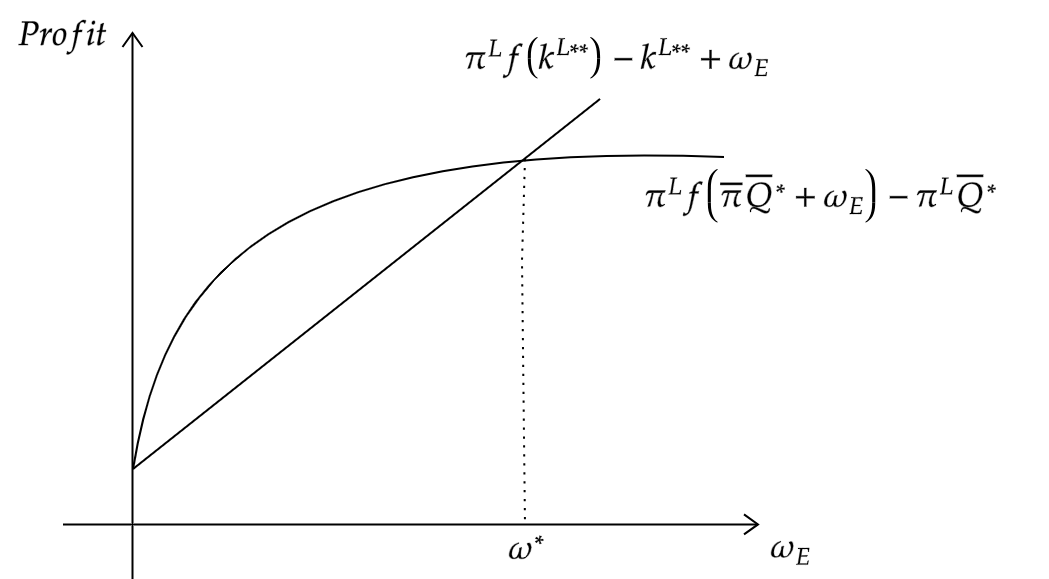
\includegraphics[width=0.5\linewidth]{pic/pool.png}
		\caption{混同均衡域}
	\end{figure}
\end{frame}

\begin{frame}{结论与讨论}
	\begin{itemize}
		\item 分离均衡结果显示,企业自身资金禀赋有限的前提下,银企经营目标差异导致了结果上的逆向选择
		\item 混同均衡条件下,银行能接受的最低回报为${{\pi }^{L}}f\left( {{k}^{L\text{**}}} \right)-{{k}^{L\text{**}}}+{{\omega }_{E}}$,即全部低质量项目的期望回报与企业初始资金之和。
		\item 但随着企业初始资金规模增大,企业越来越倾向于储蓄资金用以平滑投资,最终导致混同均衡无解。
	\end{itemize}
\end{frame}

\section{解决逆向选择:无监管市场与宏观调控}
\subsection{无监管市场假定}
\begin{frame}
	无监管市场只有一个参数$Q_{N}\in\left[0,N\right]$。均衡利率$R$标准化为1,均衡价格为$p_{Q_{N}}$。假定无监管市场具有非排他性,任意出借人都能按出资比例要求收益。
	\begin{itemize}
		\item 无监管市场只有混同均衡。而且无监管市场均衡价格$p_{Q_{N}}$不超过$\bar{\pi}$。
		\item 无监管市场不要求$\omega$,所以允许策略性违约。
		\item 因此,即使$p_{Q_{N}}<\pi^L$,也有预期违约的企业进入。
		因此企业在无监管市场融资后,将所得资金投入生产的可行集为


	\end{itemize}
	$${{\pi }^{j}}\left[ f\left( {{p}_{\left( Q,\omega  \right)}}Q+\omega  \right)-Q \right]+\mathop{\int }_{{{\text{ }\!\!\Omega\!\!\text{ }}_{N}}}\max \left\{ \left( {{p}_{{{Q}_{N}}}}-{{\pi }_{j}} \right),0 \right\}{{Q}_{N}}-\omega \ge \mathop{\int }_{{{\text{ }\!\!\Omega\!\!\text{ }}_{N}}}{{p}_{{{Q}_{N}}}}{{Q}_{N}}$$
	即企业如果将无监管市场融入的资金作为进入更高质量的、有监管市场的门槛,最低要求是融资成本大于违约收益。
	
\end{frame}

\begin{frame}{策略性违约}
	如果投资规模没有被扭曲,企业第一最优融资规模为$\frac{k^{j**}}{\pi^j}$。\\
	企业能在无监管市场上融入的资金量为
	$$Q_{N}^{j}=f\left( {{k}^{j\text{**}}} \right)-\frac{{{k}^{j\text{**}}}}{{{\pi }^{j}}}$$
	一方面,企业最优投资规模$ {k}^{j\text{**}} $不受资金禀赋限制,另一方面,企业达到最优投资规模后不会继续融资。假定$Q_{N}^{H}<\mathop{\int }_{{{\text{ }\!\!\Omega\!\!\text{ }}_{N}}}{{Q}_{N}}$
	设定$\theta_{i,Q_N}\in \left\{0,1\right\}$为是否违约的虚拟变量。
	$q_{i,Q_N}^{-}$为无内部监管市场的总信贷资金需求,有
	$${{R}_{{{Q}_{N}}}}=\left[ \frac{{{\pi }^{H}}\mathop{\int }_{i\in I_{E}^{H}}\left( 1-{{\theta }_{i,{{Q}_{N}}}} \right)q_{i,{{Q}_{N}}}^{-}+{{\pi }^{L}}\mathop{\int }_{i\in I_{E}^{L}}\left( 1-{{\theta }_{i,{{Q}_{N}}}} \right)q_{i,{{Q}_{N}}}^{-}}{{{p}_{{{Q}_{N}}}}\mathop{\int }_{i\in {{I}_{E}}}q_{i,{{Q}_{N}}}^{-}} \right]$$
\end{frame}

\begin{frame}{不活跃市场}
	外部参与者会在不活跃的无监管市场上提出融资金额为$Q_N\left(n\right)$的合同,成功率为$\pi^H$\\
	定义无监管市场的资金供给总量$ q_{i,{{Q}_{N}}}^{+} $\\
	有关有监管的不活跃市场假定仍然成立。
	

\end{frame}

\subsection{混合市场竞争性均衡}

\begin{frame}{混合市场均衡}
	\textbf{定义2:混合市场均衡}\\
	对于投融资决策集合$\left\{ q_{i,\left( Q,\omega  \right)}^{+},q_{i,\left( Q,\omega  \right)}^{-},q_{i,{{Q}_{N}}}^{+},q_{i,{{Q}_{N}}}^{-} \right\}$、违约决策$\left\{ {{\theta }_{i,{{Q}_{N}}}} \right\}$和市场价格序列$\left\{ {{p}_{\left( Q,\omega  \right)}},{{p}_{{{Q}_{N}}}} \right\}$,混合市场均衡满足//
	\begin{itemize}
		\item[1] 有监管市场满足排他性
		\item[2] 可行性。有监管市场借款时,企业使用自有资金的总投资额不超过企业能获取的总资金额度$\omega \le {{\omega }_{E}}={{p}_{{{Q}_{N}}}}\mathop{\int }_{i\in {{I}_{E}}}q_{i,{{Q}_{N}}}^{-}$。
		\item[3] 最优性。在$R_{Q_N}$和$R_{\left(Q,\omega\right)}$均成立的情况下,企业以收益最大化为目标。
		\item[4] 市场出清,即$\mathop{\int }_{i\in I_{E}^{H}}q_{i,\left( Q,\omega  \right)}^{+}=\mathop{\int }_{i\in I_{E}^{L}}q_{i,\left( Q,\omega  \right)}^{-}$,		$\mathop{\int }_{i\in I_{E}^{H}}q_{i,{{Q}_{N}}}^{+}=\mathop{\int }_{i\in I_{E}^{L}}q_{i,{{Q}_{N}}}^{-}$
	\end{itemize}
\end{frame}

\begin{frame}{混合市场一般竞争性均衡}
	\textbf{命题3 混合市场一般竞争性均衡}\\
	对于包含有监管市场$\left( Q,\omega  \right)\in \text{ }\!\!\Omega\!\!\text{ }$和无监管市场${{Q}_{N}}\in {{\text{ }\!\!\Omega\!\!\text{ }}_{N}}$的混合市场而言,假定企业部门不存在初始资金,即${{e}_{E}}=0$, 命题1和2均在混合市场满足${{\omega }_{E}}=0$时成立;在任何混合市场一般竞争性均衡中,所有无监管市场都是不活跃的,即
	$$q_{i,{{Q}_{N}}}^{-}=q_{i,{{Q}_{N}}}^{+}=0$$
	$${{p}_{{{Q}_{N}}}}\in \left( 0,{{\pi }_{L}} \right]$$
	对于任何$i\in I,{{Q}_{N}}\in {{\text{ }\!\!\Omega\!\!\text{ }}_{N}}$恒成立。\\
	此时,无论企业从无监管市场上为低质量项目融资并使用存储技术,或是从有监管市场为低质量项目借款并按合同约定投资,两种选项是无差异的。\\
	因为允许违约,贷款人不活跃;包含外部代理人,价格不为0;价格$p$在等于$ {\pi }_{L} $时,无监管市场不活跃。
\end{frame}

\begin{frame}{无违约竞争性均衡}
	\textbf{命题4 无违约竞争性均衡}\\
	对于包含有监管市场$\left( Q,\omega  \right)\in \text{ }\!\!\Omega\!\!\text{ }$和无监管市场${{Q}_{N}}\in {{\text{ }\!\!\Omega\!\!\text{ }}_{N}}$的混合市场而言,\\
	1.有监管市场$\left( Q,\omega  \right)\in \text{ }\!\!\Omega\!\!\text{ }$中,均衡序列与命题1中的分离均衡一致,但${{\omega }_{E}}$则由无监管市场最优借款额定义:
	$${{Q}^{{{H}^{\text{*}}}}}=\frac{{{k}^{H\text{**}}}-{{\omega }_{E}}}{{{\pi }^{H}}},{{\omega }_{E}}=\bar{\pi }Q_{N}^{\text{*}}$$
	2.在无监管市场${{Q}_{N}}\in {{\text{ }\!\!\Omega\!\!\text{ }}_{N}}$中,混同均衡点$q_{i,{{Q}_{N}}}^{-}$满足
	$$q_{i,{{Q}_{N}}}^{-}=\left\{ \begin{matrix}
		Q_{N}^{\text{*}} & {{Q}_{N}}=Q_{N}^{\text{*}}  \\
		0 &  else \\
	\end{matrix} \right.$$

\end{frame}

\begin{frame}{无违约竞争性均衡}
	此时混同均衡合同价格${{p}_{Q_{N}^{*}}}=\bar{\pi }$,$Q_{N}^{*}$为无内部监管市场中最优总借款额,由激励相容条件定义,即
	$$Q_{N}^{\text{*}}=\frac{\left( {{\pi }^{L}}f\left( {{k}^{H\text{**}}} \right)-\frac{{{\pi }^{L}}}{{{\pi }^{H}}}{{k}^{H\text{**}}} \right)-\left( {{\pi }^{L}}f\left( {{k}^{L\text{**}}} \right)-{{k}^{L\text{**}}} \right)}{\bar{\pi }\left( 1-\frac{{{\pi }^{L}}}{{{\pi }^{H}}} \right)}$$
	3.不活跃的无监管市场${{Q}_{N}}\in {{\text{ }\!\!\Omega\!\!\text{ }}_{N}},{{Q}_{N}}\ne Q_{N}^{\text{*}}$满足${{p}_{{{Q}_{N}}}}\in \left( 0,{{\pi }^{L}} \right]$,
	$$\mathop{\int }_{{{\text{ }\!\!\Omega\!\!\text{ }}_{N}}}{{p}_{{{Q}_{N}}}}{{Q}_{N}}={{\pi }^{L}}f\left( {{k}^{L\text{**}}} \right)-{{k}^{L\text{**}}}-\left( \bar{\pi }-{{\pi }^{L}} \right)Q_{N}^{\text{*}}$$
	4.均衡不包括违约,即当且仅当$Q_{N}^{\text{*}}<Q_{N}^{L}$时,有${{d}_{i,Q_{N}^{\text{*}}}}=0$。
\end{frame}

\begin{frame}{无违约的进一步讨论}
	如果假定无违约,那么研究借贷行为就没有意义了。\\
	如何让企业自发无违约,而不是在监管下无违约?\\
	无违约要求在$ \bar{\pi}=p_{Q_N} $的情况下有$ Q_{N}^{*} <Q_{N}^{L} $即低质量企业可以通过从无监管市场上融资并获利。结合$ Q_{N}^{*}$的定义,要满足这一条件,有
	$$Q_{N}^{*}=\frac{\left( {{\pi }^{L}}f\left( {{k}^{H**}} \right)-\frac{{{\pi }^{L}}}{{{\pi }^{H}}}{{k}^{H**}} \right)-\left( {{\pi }^{L}}f\left( {{k}^{L**}} \right)-{{k}^{L**}} \right)}{\bar{\pi }\left( 1-\frac{{{\pi }^{L}}}{{{\pi }^{H}}} \right)}<f\left( {{k}^{L**}} \right)-\frac{{{k}^{L**}}}{{{\pi }^{L}}}$$
	即
	$$\frac{Q_{N}^{H}}{Q_{N}^{L}}-1<\bar{\pi }\left( \frac{1}{{{\pi }^{L}}}-\frac{1}{{{\pi }^{H}}} \right)$$
	只需的$ \bar{\pi}=p_{Q_N} $最小值满足上式,即可达成无违约。
\end{frame}

\begin{frame}{交叉补贴}
	中间人为两类企业提供贷款,为高质量项目提供$k^H$的贷款,为低质量项目提供$k^L$的贷款,并分别在项目成功后要求$\frac{k^H}{\pi^H}$和$\frac{k^L}{\pi^L}$的回报。且要求高质量项目支付一笔交叉补贴$T$。最优化问题:
	$$\begin{matrix}
		\underset{{{k}^{H}}.{{k}^{L}},T}{\mathop{\max }}\,{{\varepsilon }^{H}}\left[ {{\pi }^{H}}f\left( {{k}^{H}} \right)-{{k}^{H}}-{{\pi }^{H}}T \right]+{{\varepsilon }^{L}}\left[ {{\pi }^{L}}f\left( {{k}^{L}} \right)-{{k}^{L}}+\frac{{{\varepsilon }^{H}}}{{{\varepsilon }^{L}}}{{\pi }^{L}}T \right]+e  \\
	\end{matrix}$$
	s.t.
	$$\begin{matrix}
		{{\pi }^{L}}f\left( {{k}^{H}} \right)-\frac{{{\pi }^{L}}}{{{\pi }^{H}}}{{k}^{H}}-{{\pi }^{L}}T\le {{\pi }^{L}}f\left( {{k}^{L}} \right)-{{k}^{L}}-\frac{{{\varepsilon }^{H}}}{{{\varepsilon }^{L}}}{{\pi }^{H}}T  \\
	\end{matrix}$$
	$$\begin{matrix}
		{{\pi }^{H}}f\left( {{k}^{L}} \right)-\frac{{{\pi }^{H}}}{{{\pi }^{L}}}{{k}^{L}}+\frac{{{\varepsilon }^{H}}}{{{\varepsilon }^{L}}}{{\pi }^{H}}T\le {{\pi }^{H}}f\left( {{k}^{H}} \right)-{{k}^{H}}-{{\pi }^{H}}T  \\
	\end{matrix}$$
\end{frame}

\begin{frame}
	\textbf{命题5 交叉补贴均衡}
	假定企业部门自有资金为0,中间人的最优决策满足
	$${{k}^{j}}={{k}^{j**}},j\in \left\{ H,L \right\}$$
	$$T=\frac{{{\varepsilon }^{L}}}{\varepsilon }\left[ \frac{{{\pi }^{L}}f\left( {{k}^{H**}} \right)-\frac{{{\pi }^{L}}}{{{\pi }^{H}}}{{k}^{H**}}-{{\pi }^{L}}f\left( {{k}^{L**}} \right)-{{k}^{L**}}}{{\bar{\pi }}} \right]$$
	
\end{frame}


\section{总结与政策建议}

\begin{frame}{总结}
	\begin{itemize}
		\item[1] 数字化转型项目风险会引起外部利益相关者担忧。
		\item[2] 数字化转型导致信贷市场逆向选择是在融资约束下的市场理性结果。
		\item[3] 建设多层次资本市场、放松企业融资约束能缓解信贷逆向选择。
		\item[4] 通过实施交叉补贴,市场主体能有效识别企业是否具有稳健经营能力。
	\end{itemize}
\end{frame}
\begin{frame}
	\begin{itemize}
		\item 平衡数字化转型与主业经营
		\item 畅通融资渠道、增加模仿成本
		\item 政府补贴引导企业内部补贴
	\end{itemize}
\end{frame}
\begin{frame}
    \begin{center}
        {\Huge\calligra Thanks!}
    \end{center}
\end{frame}

\section{文章评述}

\begin{frame}{总结与主要看点}
	\begin{itemize}
		\item[1] 数字化转型能否促进绿地投资?
		\begin{itemize}
			\item[] 跨国企业数字化转型显著促进了企业绿地投资,表现为绿地投资在总OFDI中的占比更多
		\end{itemize}
		\item[]
		\item[2] 数字化转型如何促进绿地投资?
		\begin{itemize}
			\item[] 交易成本渠道:降低交易成本促进绿地投资
			\item[] 生产效率渠道:提升生产效率促进绿地投资
			\item[] 海外资产存量渠道:降低海外资产促进绿地投资
		\end{itemize}
	\end{itemize}
\end{frame}

\begin{frame}{OFDI模式选择与bargaining power的思考}
	
	\begin{itemize}
		\item[1] 起源于逻辑排他的思考,安全审查只是讨价还价能力的体现。
		\item[2] 正向逻辑:数字技术缓解并购双方信息不对称、提升识别能力
		\begin{itemize}
			\item[] 然而,结论似乎并不是想象中的那样?
		\end{itemize}
		\item[3] 数字技术如何影响谈判过程中并购与反并购行为?
		\begin{itemize}
			\item[] 并购方可以运用数字技术缓解信息不对称
			\item[] 反并购方可以释放噪声,使成交均值偏移并购方期望以获益
		\end{itemize}
		\item[4] 并购中的信息结构
		\begin{itemize}
			\item[] 反并购方也可以针对并购方期望,反向设置信息结构
			\item[] 如果将被并购企业视为卖家,并购企业视为买家,那么设置信息结构就是被并购企业对并购企业实施三级价格歧视。
		\end{itemize}
	\end{itemize}

\end{frame}
\begin{frame}{技术上的反思}
	\begin{itemize}
		\item[1] 权宜之计的词频:“言行不一”但又难以替代\\~\\
		\item[2] 什么会影响OFDI?企业特质、管理层特征等都会影响OFDI。控制个体异质性有其必要性。\\
		\begin{itemize}
			\item[] 企业数字化转型也是一企一策,或者专门交给第三方,而非云平台。
		\end{itemize}
		\item[3] 数字化转型驱动的OFDI结构转型,使企业更接近客户了吗?
			\item[] 如果是出口企业,至少在地理距离上是的。
			\item[] 绿地投资的适应过程中存在摩擦。
	\end{itemize}
\end{frame}
\end{document}